\documentclass[20pt,margin=1in,innermargin=-4.5in,blockverticalspace=-0.25in]{tikzposter}
\geometry{paperwidth=42in,paperheight=30in}
\usepackage[utf8]{inputenc}
\usepackage{csquotes}
% \usepackage[estonian]{babel}
\usepackage{amsmath}
\usepackage{amsfonts}
\usepackage{amsthm}
\usepackage{amssymb}
\usepackage{mathrsfs}
\usepackage{enumitem}
\usepackage{graphicx}
\usepackage{adjustbox}
\usepackage{xcolor}
\usepackage[backend=biber,style=numeric]{biblatex}
\usepackage{CIMAT}
%\usepackage{subfigure}

%Declarations
\newtheorem{theorem}{Teorema}[section]
\newtheorem*{proposition}{Proposici\'on}
\newtheorem{corollary}[theorem]{Corolario}
\newtheorem{lemma}[theorem]{Lema}
\newtheorem*{definition}{Definici\'on}
\newtheorem*{remark}{Observaci\'on}
\newtheorem*{ejemplo}{Ejemplo}
\newtheorem{claim}[theorem]{Claim}
\newtheorem{conjecture}[theorem]{Conjetura}
\newtheorem*{conjecture*}{Conjetura}
\newtheorem*{theorem*}{Teorema}
\newtheorem*{lemma*}{Lema}

\newcommand{\Aut}{\operatorname{Aut}\nolimits}
\newcommand{\alg}{\operatorname{Alg}\nolimits}
\newcommand{\sete}{\operatorname{Set}\nolimits}
\newcommand{\Coker}{\operatorname{Coker}\nolimits}
\newcommand{\colim}{\operatorname{colim}\nolimits}
\newcommand{\hocolim}{\operatorname{hocolim}\nolimits}
\newcommand{\Hom}{\operatorname{Hom}\nolimits}
\newcommand{\ide}{\operatorname{id}\nolimits}
\newcommand{\me}{\operatorname{m}\nolimits}
\newcommand{\Ind}{\operatorname{Ind}\nolimits}
\newcommand{\inv}{\operatorname{inv}\nolimits}
\newcommand{\Ima}{\operatorname{Im}\nolimits}
\newcommand{\Inj}{\operatorname{Inj}\nolimits}
\newcommand{\Inn}{\operatorname{Inn}\nolimits}
\newcommand{\Iso}{\operatorname{Iso}\nolimits}
\newcommand{\Ker}{\operatorname{Ker}\nolimits}
\newcommand{\Out}{\operatorname{Out}\nolimits}
\newcommand{\Syl}{\operatorname{Syl}\nolimits}
\newcommand{\Rep}{\operatorname{Rep}\nolimits}
\newcommand{\Res}{\operatorname{Res}\nolimits}
\newcommand{\Top}{\operatorname{Top}\nolimits}
\newcommand{\grup}{\operatorname{Grp}\nolimits}
\newcommand{\nat}{\operatorname{Nat}\nolimits}

\usepackage{mwe} % for placeholder images

\addbibresource{ref.bib}

% set theme parameters
\tikzposterlatexaffectionproofoff
\usetheme{CIMATTheme}
\usecolorstyle{CIMATStyle}

\usepackage[scaled]{helvet}
\renewcommand\familydefault{\sfdefault} 
\renewcommand{\vec}[1]{\bm{#1}}
\newcommand{\Tr}{\text{Tr}}
\usepackage[T1]{fontenc}

\title{Teoría de Kolmogorov para flujos turbulentos}
\author{\textbf{César Isaí García Cornejo}\textsuperscript{1} \& \textbf{José Ulises Márquez Urbina}\textsuperscript{2} }

\institute{\textsuperscript{1} Universidad de Guadalajara, U de G  \\ \textsuperscript{2}Centro de Investigaci\'on en Matem\'aticas, CIMAT, A.C. }
\titlegraphic{
\includegraphics[width=0.05\linewidth]{logoCIMAT.jpg}}

% begin document
\begin{document}
\maketitle
\centering
\begin{columns}
    \column{0.32}
    \block{Introducción}{
        En mecánica de fluidos, la turbulencia es el término usado para hacer mención de aquellos flujos caóticos con movimientos complejos difícilmente predecibles. Esta posee características tales como la \textbf{disipación de la energía}, es altamente \textbf{difusiva}, el campo de velocidad tiene comportamiento \textbf{multiescala}, entre otras.
        
     	\vspace{1cm}
     	\begin{center}
     	    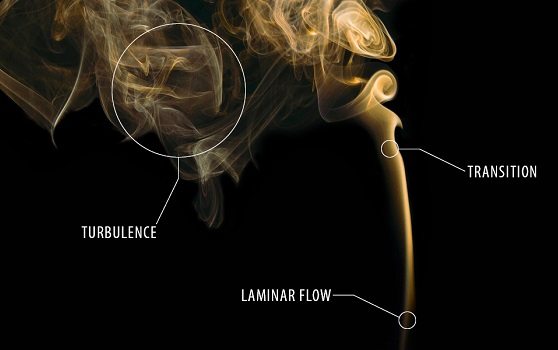
\includegraphics[width=0.25\textwidth ]{figuras/Laminar-turbulent-flow.jpg}
     	\end{center}
        
        \vspace{1cm}
        La dinámica del campo de velocidad de los flujos turbulentos es descrita por la ecuación de \textbf{Navier-Stokes}, sin embargo no es tarea sencilla dar con la solución que dicho modelo provee. Para superar dicha dificultad, se pretende introducir al espectador a la modelación estocástica del campo de velocidad usando conceptos de teoría de la probabilidad tal como el \textbf{campo aleatorio}. La \textbf{teoría K41} de Kolmogorov fue aplaudida por ser la primera en dar una correcta comprensión de los flujos turbulentos, esta se fundamente en establecer relaciones para los momentos considerando al campo de velocidad como un campo aleatorio, los detalles serán esbozados a lo largo del desarrollo. Finalmente, se presenta el método para desarrollar modelos fenomenológicos para este tipo de flujos.
		
       
    }
         
    \block{Acercamiento Físico}{
         Consideremos flujos turbulentos incompresibles, entonces la dinámica del campo de velocidad $\boldsymbol{v}$ es descrita por la \textbf{ecuación de Navier-Stokes} para flujos incompresibles
		\begin{align}
            \frac{\partial \boldsymbol{v}}{\partial t}+\boldsymbol{v}\cdot \nabla\boldsymbol{v}&=-\nabla p + \nu\nabla ^{2}\boldsymbol{v}+\boldsymbol{f},
            \label{1.01}\\
            \nabla \cdot \boldsymbol{v} &= 0.
            \label{1.02}
        \end{align}
        Observemos que estas poseen algunas \textbf{simetrías}, por nombrar algunas tenemos la \textbf{simetría translacional} que nos permite hacer el cambio
        \begin{align}
            t,\boldsymbol{r},\boldsymbol{v} \mapsto t,\boldsymbol{r}+\boldsymbol{\rho}, \boldsymbol{v},
        \end{align}
        para todo $\boldsymbol{\rho} \in \mathbb{R}^3$ y el campo de velocidad seguirá satisfaciendo (\ref{1.01}). 
        
		Ahora es natural hablar sobre \textbf{leyes de conservación}, haciendo un análisis a la ecuación de Navier-Stokes (funciones periódicas) nos encontramos que existe la \textbf{conservación del momento} tras promediar $\boldsymbol{v}$, esta relación se expresa 
		\begin{align}
		    \frac{d}{dt} \left\langle \boldsymbol{v}\right \rangle = 0.
		\end{align}
		}
		
		\column{0.36}
		
		\block{}{
		Además podemos dar con la relación
		\begin{align}
		    \frac{\mathrm{d} }{\mathrm{d} t}\left \langle \frac{1}{2} v^{2} \right \rangle= -\nu \left \langle \left | \boldsymbol{\omega} \right | ^{2}\right \rangle,
            \label{2.02}
		\end{align}
		que es la ecuación de \textbf{balance de energía global} con $\boldsymbol{\omega}=\nabla \times \boldsymbol{v}$. Sin embargo el \textbf{término de advección} (no lineal) de la ecuación de Navier-Stokes no interviene en la deducción de (\ref{2.02}).
		
		Para conocer la contribución del término de advección es necesario introducir la idea de \textbf{escala}. Para una función arbitraria $f$ periódica, expresada en series de Fourier de la forma
		\begin{align}
            f(\boldsymbol{r})= \sum_{k}\hat{f}_ke^{i\boldsymbol{k}\cdot \boldsymbol{r}}, \:\:\:\:\:\:\:\:\:\:\:\: \boldsymbol{k}\in \frac{2\pi}{L}\boldsymbol{Z}^{3},
            \label{3.1}
        \end{align}
        a cada $\boldsymbol{k}$ se le asocia un escala $l\sim K^{-1}$. Llamemos filtrado bajo a la serie de Fourier truncada
        \begin{align}
            f^{\textless}_{K}(\boldsymbol{r})= \sum_{k\leq K}\hat{f}_ke^{i\boldsymbol{k}\cdot \boldsymbol{r}},
        \end{align}
        aplicando el concepto a (\ref{1.01}) obtenemos
        \begin{align}
            \partial_t \mathcal{E}_K + \Pi_K = -2\nu\Omega_K+\mathcal{F}_K,
            \label{3.8}
        \end{align}
		que es la ecuación de \textbf{balance de energía escala por escala}.
		\begin{center}
		   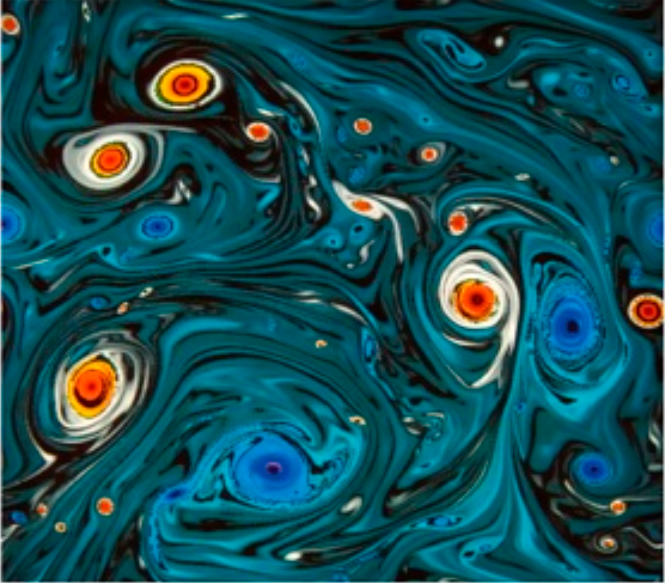
\includegraphics[width=0.15\textwidth ]{figuras/vortices.png}
		\end{center}
		}
    
    \block{Campos Aleatorios}{
    
        \textbf{Definición:} Dado un espacio de probabilidad $(\Omega,\mathcal{F},P)$ y dado un espacio geométrico $M$ (variedad), un \textbf{campo aleatorio} $X$ en este espacio de probabilidad sobre $M$ es una colección de variables aleatorias 
        \vspace{-0.5cm}
        \begin{align}
            \{ X(m): m\in M\}.
            \label{13.30}
        \end{align}
        En el caso $X\in \mathbb{R}^N$, decimos que $X$ una \textbf{función aleatoria} si $ N=1$ en cualquier otro caso es un campo aleatorio. Mencionaremos el campo aleatorio (N,d) para el campo aleatorio en $\mathbb{R}^N$ que toma valores en $\mathbb{R}^d$. Consideremos un campo aleatorio  $X(r) \in \mathbb{R}$, $r\in\mathbb{R}^d$, $\omega \in \Omega$. Para comenzar tomemos el caso unidimensional (N=1), es decir, la función aleatoria $X$ siendo \textbf{homogéneo e isotrópico}
        \begin{align}
            \left \langle X(r_1)X(r_2) \right\rangle = \left \langle X(gr_1)X(gr_2) \right\rangle,
            \label{11.01}
        \end{align}
        con $g \in G$ el grupo de translaciones y rotaciones de $\mathbb{R}^d$. En el caso \textbf{estacionario}
        se satisface
        \vspace{-0.5cm}
        \begin{align}
            \left\langle X(r) \right \rangle = \mu, \:\:\:\:\:\:\:\:    \left \langle X(r_1)X^*(r_2) \right \rangle = C(|r_1-r_2|),
        \end{align}
        donde $C$ es la \textbf{función de correlación}.
    
    }

    
    
    \column{0.32}
    \block{Descripción Estocástica}{
        Se ha notado experimentalmente que el campo de velocidad de flujos turbulentos muestran comportamientos que cercanos a los campos aleatorios.
        \begin{center}
     	    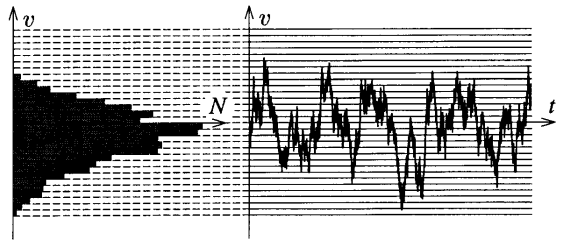
\includegraphics[width=0.25\textwidth ]{figuras/histo.png}
     	\end{center}
        Consideremos el campo de velocidad $\boldsymbol{v}(t,\boldsymbol{r},\bar{\omega})$, solución de la ecuación de Navier-Stokes con condición inicial $\bar{\omega}$, como un campo aleatorio. Definimos los \textbf{momentos} del campo de velocidad $\boldsymbol{v}$ de orden m como
        \begin{align}
             \left \langle v_{i_{1}}(t_{1},\boldsymbol{r}_{1}) v_{i_{2}}(t_{2},\boldsymbol{r}_{2})\cdot \cdot \cdot v_{i_{m}}(t_{m},\boldsymbol{r}_{m}) \right \rangle,
             \label{5.01}
        \end{align}
        el \textbf{tensor de correlación} para un campo aleatorio estacionario y homogéneo
        \begin{align}
            \left \langle v_i(t,\boldsymbol{r})v_j(t',\boldsymbol{r'}) \right \rangle = \Gamma_{ij}(t-t',\boldsymbol{r}-\boldsymbol{r'}).
            \label{5.08}
        \end{align}
        por el \textbf{teorema de Bochner} se tiene la representación espectral
        \begin{align}
            v(t,\bar{\omega})=\int _{\mathbb{R}}e^{ift}\hat{v}(f,\bar{\omega})df, \:\:\:\: \mathcal{E}(F)\equiv\frac{1}{2}\left \langle \left [ v^{\textless }_{F}(t) \right ]^{2} \right \rangle, \:\:\:\:\:\: E(f)\equiv\frac{\mathrm{d} }{\mathrm{d} f}\mathcal{E}(f)\geq 0.
        \end{align}
        % se define el \textbf{espectro acumulado de energía} 
        % \begin{align}
        %     \mathcal{E}(F)\equiv\frac{1}{2}\left \langle \left [ v^{\textless }_{F}(t) \right ]^{2} \right \rangle, \:\:\:\:\:\: E(f)\equiv\frac{\mathrm{d} }{\mathrm{d} f}\mathcal{E}(f)\geq 0.
        % \end{align}
        
        \vspace{-0.75cm}
        por ajuste a los datos experimentales
        \begin{align}
        E(k)\propto k^{-\frac{5}{3}}, \:\: \: \:\:\:     \left \langle |\boldsymbol{v}(\boldsymbol{r}')- \boldsymbol{v}(\boldsymbol{r})|^{2} \right \rangle\propto |\boldsymbol{r}'-\boldsymbol{r}|^{2/3},
            \label{7.6}
        \end{align}
        que es \textbf{la ley 2/3}. Definiendo la \textbf{función de estructura}
        \begin{align}
            S_p(l)\equiv \left \langle \left ( \delta v_{||}(l) \right )^{p} \right \rangle, \:\:\:\:\: \delta v_{||}(\boldsymbol{r+l})\equiv \left [ \boldsymbol{v}(\boldsymbol{r}+\boldsymbol{l})-v(\boldsymbol{r}) \right ]\cdot \frac{\boldsymbol{l}}{l}.
            \label{8.01}
        \end{align}
        Partiendo de la ecuación de Navier-Stokes se puede mostrar \cite{frisch1995turbulence}
        \begin{align}
            S_3(l)=-\frac{4}{5}\varepsilon l,
            \label{8.10}
        \end{align}
        que es la \textbf{ley 4/5}. Por auto-similitud se puede inferir \cite{birnir2013kolmogorov}
        \begin{align}
            S_p(l)=C_p(\varepsilon l)^{p/3}.
            \label{9.11}
        \end{align}
        Por último, la representación espectral para el proceso Y es 
        \begin{align}
            v(t) = \int_{-\infty}^{\infty}(e^{i\lambda t}-1) Z(d\lambda) + ut + v, \:\:\:\:\: S(l) = 2\int_{\mathbb{R}/ \{ 0\}} (1- cos\lambda l) \Phi(d\lambda) + al^2
        \end{align}
        % \vspace{-0.5cm}
        con $S(l)$ que es la función de correlación del incremento del campo de velocidades.
    }
    
    \vspace{-0.1cm}
    \block{References}{
        \vspace{-1em}
        \begin{footnotesize}
        \printbibliography[heading=none]
        \end{footnotesize}
    }
\end{columns}
\end{document}